\documentclass{report}

\input{~/latex/template/preamble.tex}
\input{~/latex/template/macros.tex}

\title{\Huge{Chapter 2 Notes - Statistics}}
\author{\huge{Matt Warner}}
\date{\huge{}}
\pagestyle{fancy}
\fancyhf{}
\rhead{}
\lhead{\leftmark}
\cfoot{\thepage}
% \usepackage[default]{sourcecodepro}
% \usepackage[T1]{fontenc}

\usepackage{tikz}
\usepackage{pgfplots}
\pgfplotsset{compat=1.18}

\pgfpagesdeclarelayout{boxed}
{
  \edef\pgfpageoptionborder{0pt}
}
{
  \pgfpagesphysicalpageoptions
  {%
    logical pages=1,%
  }
  \pgfpageslogicalpageoptions{1}
  {
    border code=\pgfsetlinewidth{1.5pt}\pgfstroke,%
    border shrink=\pgfpageoptionborder,%
    resized width=.95\pgfphysicalwidth,%
    resized height=.95\pgfphysicalheight,%
    center=\pgfpoint{.5\pgfphysicalwidth}{.5\pgfphysicalheight}%
  }%
}

\pgfpagesuselayout{boxed}

\begin{document}
  \maketitle

\begin{large}
  \textbf{\section{Types of Data}} 
\end{large}
\bigbreak \noindent \bigbreak \noindent
\begin{large}
  \textbf{\underline{Terminology}} 
\end{large}
\bigbreak \noindent
\begin{itemize}
  \item If we measure or record 
  \begin{itemize}
    \item one oberservation from each individual or object we have \textbf{\underline{univariate data}}
    \item two oberservations from each individual or object we have \textbf{\underline{bivariate data}}
    \item more than two oberservations from each individual or object we have \textbf{\underline{multivariate data}} \\ (e.g. height, weight, gender, blood presure, and cholesterol level of each person)
  \end{itemize}
\item Types of Data
  \begin{itemize}
    \item \textbf{\underline{Categorical or qualitative}} - non-numerical  oberservations that may be placed in categories.
    \item \textbf{\underline{Numerical or quantitative}} - observations that are numbers.
  \end{itemize}
  \item A numerical data set is
    \begin{itemize}
      \item \textbf{\underline{Discrete}} if its set of possible values is a finite set or a countable infinite set (i.e. an infinite sequence with a first value, second value, etc.)
      \item \textbf{\underline{Continuous}} if its set of possible values is an infinite set that forms an interval on the number line (usually associated with measuring)
    \end{itemize}
  \end{itemize}
\bigbreak \noindent \bigbreak \noindent
\thmcon{
  \textbf{\underline{Discrete vs Continuous}}
  \vspace{3mm}

  \textbf{Continuous Data:} \hspace{50mm} \textbf{Discrete Data:}
  \vspace{2mm}

  It can take on any value in an interval \hspace{23mm} It can only have specific values.
  \vspace{2mm}

  Data that can be measured (i.e. speed of a car) \hspace{8.5mm} Data that can be counted (i.e number of books)
}
\bigbreak \noindent 
\begin{large}
  \textbf{\section{Bar Charts and Pie Charts}} 
\end{large}
\bigbreak \noindent \bigbreak \noindent
\begin{large}
\textbf{Frequency distribution} 
\end{large}
\bigbreak \noindent
\thmcon{
  \textbf{\underline{Defintion}}
  \vspace{3mm}

  The natural summary measures for a categorical data set are the number of times each category occurred and the proportion of times each category occured. These values are usually displayed in a table as in \underline{Table 2.1}
  \vspace{3mm}

  A \textbf{frequency distrobution} for categorical data is a summary table that presents categories, counts, and proportions.
  \begin{enumerate}
    \item Each unique value in a categorical data set is a label, or class. In \underline{Table 2.1} the classes are mammals, birds, reptiles, etc.
    \item The frequency is the count for each class. In \underline{Table 2.1}, the frequency for the mammals class is 202 (i.e. 202 mammals were on the critically endangered species list.)
    \item The relative frequency, or sample proportion, for each class is the frequency of the class divided by the total number of observations.  In \underline{Table 2.1}, the relative frequency for the amphibians class is $\frac{552}{2000} = 0.276$
  \end{enumerate}
}

\begin{figure}[ht]
\centering
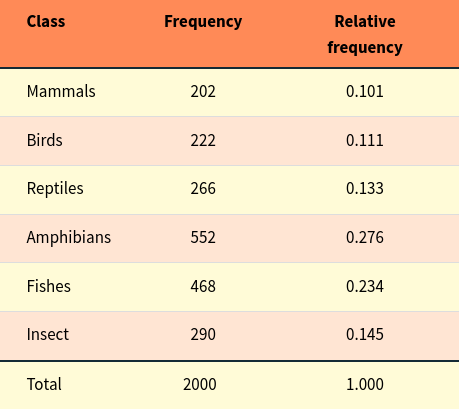
\includegraphics[width=0.5\textwidth]{ ~/niu/Stat200/figures/relfreq.png }
\caption{Table 2.1}
\end{figure}

\bigbreak \noindent \bigbreak \noindent

\begin{large}
 \noindent \textbf{Bar Charts} 
\end{large}
\bigbreak \noindent
A \textbf{\underline{Bar chart}} is a graphical representation of a frequency distribution for categorical data. An example of a bar chart is shown in \underline{Figure 2.5}.
\bigbreak \noindent 
\begin{figure}[ht]
\centering
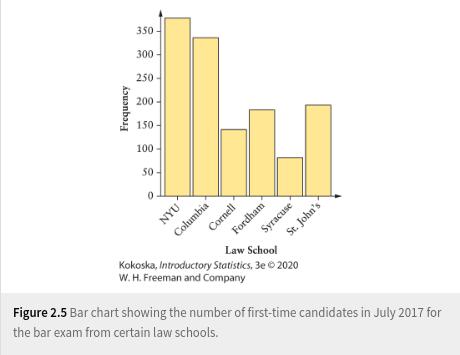
\includegraphics[width=0.5\textwidth]{ ~/niu/Stat200/figures/barchart.png }
\end{figure}

\pagebreak
\begin{large}
  \noindent \textbf{Pie Charts} 
\end{large}
\bigbreak \noindent
A \textbf{\underline{pie chart}} is another graphical representation of a frequency distribution for categorical data. An example of a pie chart is shown in \underline{Figure 2.8}
\bigbreak \noindent
\begin{figure}[ht]
\centering
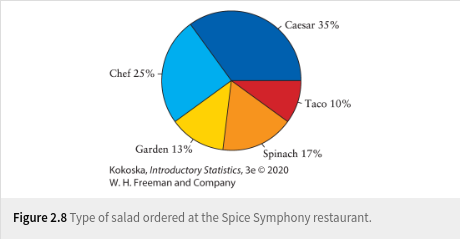
\includegraphics[width=0.5\textwidth]{ ~/niu/Stat200/figures/piechart.png }
\end{figure}
\bigbreak \noindent
\begin{large}
  \textbf{\section{Frequency Distributions and Histograms}} 
\end{large}
\bigbreak \noindent
\thmcon{
  \textbf{\underline{Defintion}}
  \vspace{3mm}

  A \textbf{frequency distribution} for numerical data is a summary table that displays classes, frequencies, relative frequencies, and cummulative relative frequencies.
}
\bigbreak \noindent
\thmcon{
  \textbf{\underline{How to Construct a Frequency Distribution for Numerical Data}}
  \vspace{3mm}

1. Choose a range of values that captures all the data. Divide it into nonoverlapping (usually equal) intervals. Each interval is called a class, or class interval. The endpoints of each class are the class boundaries.
\vspace{2mm}

2. We use the left-endpoint convention. An observation equal to an endpoint is allocated to the class with that value as its lower endpoint. Hence, the lower class boundary is always included in the interval, and the upper class boundary is never included. This ensures that each observation falls into exactly one interval.
\vspace{2mm}

3. In practice, there should be 5-20 intervals. Use friendly numbers, for example, $10-20$ and $20-30$, rather than more complicated categories, such as $15.376-18.457$ and $18.457-21.538$.
\vspace{2mm}

4. Count the number of observations in each class interval. This count is called the class frequency or simply the frequency.
\vspace{2mm}

5. Compute the proportion of observations in each class. This ratio, the class frequency divided by the total number of observations, is called the relative frequency.
}
\bigbreak \noindent
\begin{large}
  \textbf{Histograms} 
\end{large}
\bigbreak \noindent
A \underline{histogram} is a graphical representation of a frequency distrobution, a plot of frequency versus class interval. Given a frequency distrobution, here is a procedure for constructing a histogram.
\begin{enumerate}
  \item Draw a horizontal line (measurement) axis and place tick marks corresponding to the class boundaries.
  \item Draw a vertical axis and place tick marks corresponding to frequency. Label each axis.
  \item Draw a rectangle above each class with height equal to frequency.
\end{enumerate}

\pagebreak
\nt{

The shape of a distribution may be symmetric or skewed. The center of a distribution referes to the position of the majority of the data, and measures of variability indicate the spread of the data. The \textbf{\textit{variability}} (or dispersion) of a distrobution describes how much the measurements vary, as well as how compact or how spread out the data are. 
}
\bigbreak \noindent \bigbreak \noindent

\begin{LARGE}
  \noindent \textbf{Density Histograms} 
\end{LARGE}
\bigbreak \noindent
If the class widths are unequal in a frequency distribution, then neither the frequency nor the relative frequency should be used on the vertical axis of the corresponding histogram. To account for the unequal class widths, set the area of each rectangle equal to the relative frequency. In this case, the height of each rectangle is called the \textit{density}, and it is equal to the relative frequency divided by the class width.
\bigbreak \noindent

\thmcon{
  \textbf{\underline{How to find the Density}}
  \vspace{3mm}

To find the density for each class:
\begin{enumerate}
  \item Set the area of each rectangle equal to the relative frequency. \vspace{2mm} \\ The area of each rectangle is height times width  
\end{enumerate}

$$
\begin{aligned}
\text { Area of rectangle } & =\text { Relative frequency } \\
& =(\text { Height }) \times(\text { Class width })
\end{aligned}
$$
\vspace{2mm}

\hspace{3.5mm} 2. Solve for height.
\vspace{3mm}

\centerline{Density $=$ Height $=($ Relative frequency $) /($ Class width $)$}
}
\bigbreak \noindent \bigbreak \noindent \bigbreak \noindent
\begin{figure}[ht]
\centering
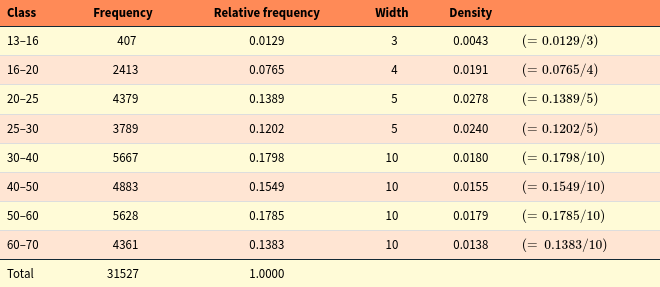
\includegraphics[width=0.89\textwidth]{ ~/niu/Stat200/figures/densityhistogram.png }
\caption{Table showing density}
\end{figure}

\pagebreak

\begin{LARGE}
\noindent \textbf{Shape of Distribution}
\end{LARGE}
\bigbreak \noindent
\begin{mdframed}
 Because the relative frequency is equal to the area of each rectangle in a density histogram, the sum of the areas of all the rectangles is 1 . This is an important concept as we begin to associate area with probability.
\bigbreak \noindent
The shape of a distribution, represented in a histogram, is an important characteristic. To help describe the various shapes, we draw a smooth curve along the tops of the rectangles that captures the general nature of the distribution (as shown in \underline{Figure 2.25}). To help identify and describe distributions quickly, a smoothed histogram is often drawn on a graph without a vertical axis, without any tick marks on the measurement axis, and without any rectangles (as shown in \underline{Figure 2.26}). 
\end{mdframed}
\vspace{3mm}

\begin{figure}[ht]
\centering
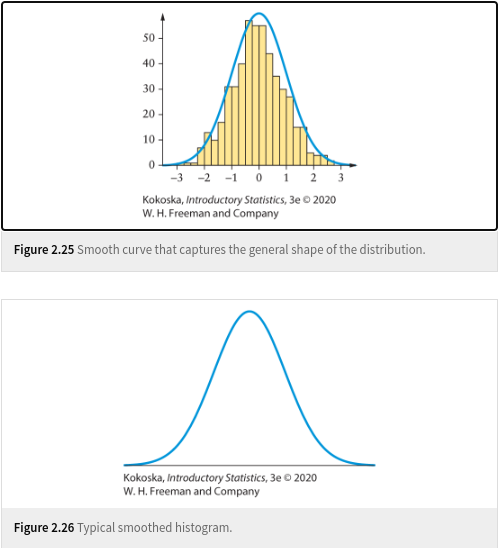
\includegraphics[width=0.65\textwidth]{ ~/niu/Stat200/figures/shape.png }
\end{figure}
\bigbreak \noindent
\thmcon{
  \textbf{\underline{Describing Peaks}}
  \vspace{3mm}
  
  \begin{enumerate}
    \item A \textbf{unimodal} distribution has \textit{one peak}. This is very common, as almost all distributions have a single peak.
    \item A \textbf{Bimodal} distribution has \textit{two} peaks. This shape is not very common but may occur if data from two different populations are accidentally mixed.
    \item A \textbf{Multimodal} distribution has more than \textit{one} peak. A distribution with more than two distinct peaks is very rare.
  \end{enumerate}
}
\pagebreak
\thmcon{
  \textbf{\underline{Further classification}}
  \vspace{3mm}

  \begin{enumerate}
    \item A unimodal distribution is \textbf{symmetric} if there is a vertical line of symmetry in the distribution.
  \end{enumerate}
}



\end{document}
